Even though a lot of visualization tools for different use cases emerged, there is only a small amount of tools trying to animate the transition between two visualizations. This chapter provides three types of exemplarily selected tools:

\begin{enumerate*}
\item tools that use some kind of animation to create the visualization,
\item tools that also allow to create maps and
\item tools that try to animate the transition when changing the visual appearance.
\end{enumerate*}

In order to evaluate all applications with the same base, the analysis framework mentioned in chapter \ref{s:basics} on page \pageref{s:basics} is used.

\subsubsection{SandDance}
\citeauthor{Drucker2015} describe a tool which makes use of so called unit visualizations. This type of visualization is best described as using one complete row of a dataset and representing it as a unit. Advantages of using units are described in the following list \iacite{Drucker2015}:
\begin{itemize}
\item \textbf{The forest and the trees:} when using a visualization based on aggregation of data, it is possible to hide outlying data or have outlying data influence the representation \iacite{Drucker2015}. However, unit visualizations maintain a one-to-one correspondence between rows in a dataset with the represenation. While classical bar charts only show one static bar for each aggregated attribute, unit visualizations show the dynamic units building that bar. Therefore, a bar for a bar chart made in a unit visualization is not a single, static shape. It is a dynamically created bar with shapes representing each unit individually and thus showing the trees yielding the forest instead of showing only the forest.

\item \textbf{Semantic constancy:} the connection between a row and a unit is maintained throughout all changes. Thus, changing visual attributes or switching from one visualization to another, does not break that bond.

\item \textbf{Direct interaction:} when using the concept of unit visualizations, it is fairly easy to show additional information of each unit by providing for example tooltips. Even when using multiple views, the concept of linking and brushing (see chapter \ref{s:linking-brushing} on page \pageref{s:linking-brushing} fore more information) can be accomplished by highlighting the selected units in every view. Furthermore, if some kind of aggregated visualization is implemented with this concept, the units can still be highlighted because they are still visible.

\item \textbf{Animation:} because of the semantic constancy, it is possible to animate smoothly between different visualizations. Transitions only update the position of every unit since they are all present.

\end{itemize}

Albeit showing a lot of advantages, the concept of unit visualizations show some weaknesses:

\begin{itemize}
\item Using a lot of units, for example, in a bar can lead to visual clutter compared to a single, static aggregated one.

\item Accessing the information of the aggregation needs more calculation in a unit visualization because each unit already represents its row and still needs to know its particular group for aggregation. First, this group needs to be calculated and second, some attributes e.g. count or sum needs to be shown in the visualization.

\item Scaling is the main weakness of this type of visualizations. Aggregate visualizations can potentially use a much larger dataset, compared to unit visualizations. Scaling does not only include the amount of data used, it also includes the hardware accessible. Displaying thousands of items and animating them requires more operation power than calculating an aggregation and drawing a rectangle on a fixed position.

\end{itemize}

\begin{figure}[!htb]
\centering
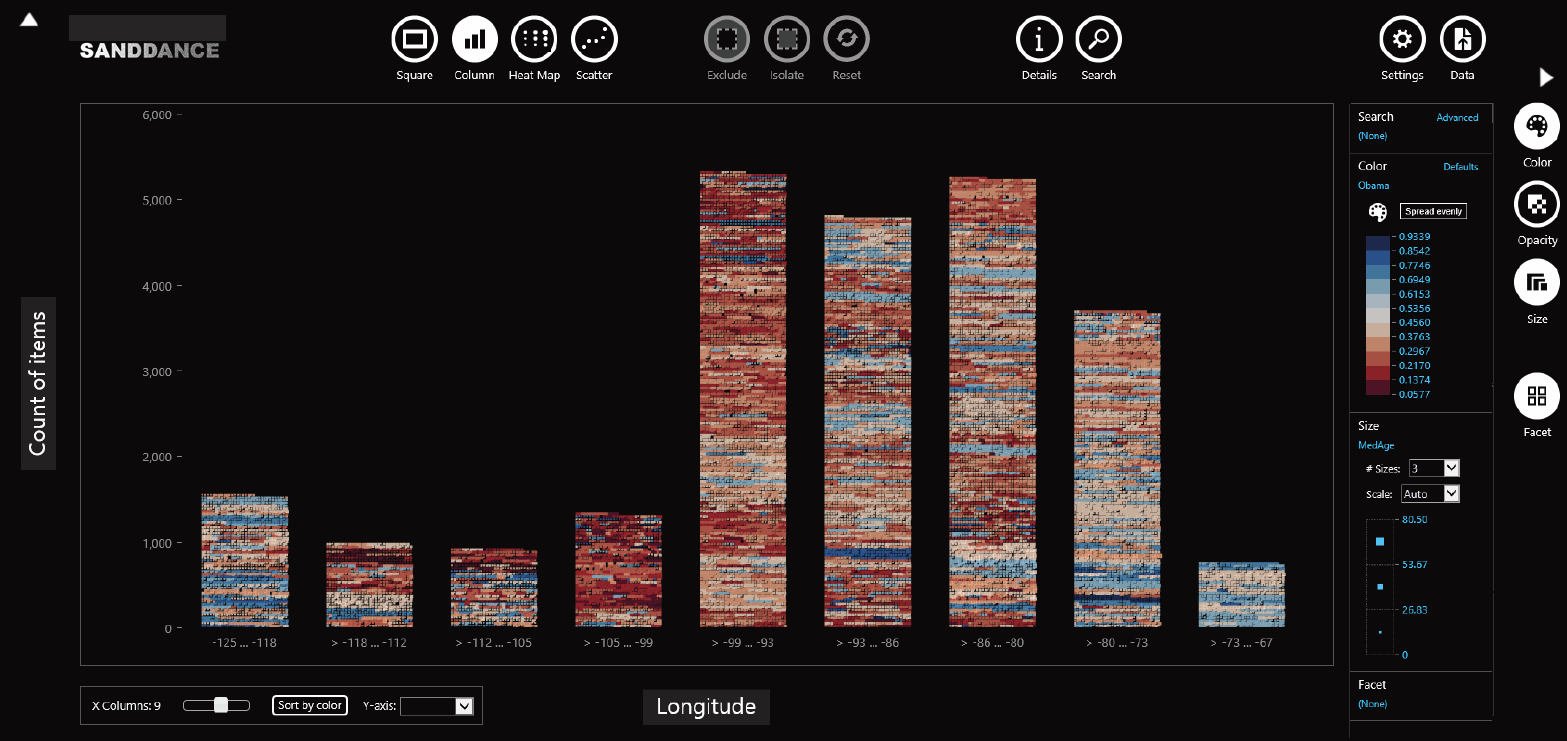
\includegraphics[width=0.8\textwidth,keepaspectratio]{images/methods/related/sanddance.png}
\caption[
    Concept of SandDance \iacite{Drucker2015}.
]{SandDance}
\label{fig:sanddance}
\end{figure}

Figure \ref{fig:sanddance} on page \pageref{fig:sanddance} shows the prototype. It allows to manually change visual channels to the right and change visual appearance e.g. changing the type of visualization at the top left. According to the analysis framework, SandDance uses static tables as input data only. \citeauthor{Drucker2015} states, that the tool was built to explore the benefits of using unit visualizations. Therefore it has no real use case to analyse, because it was used to show a completly different type of visualization without considering user benefit. However, one could say that the tool can be used to consume information and maybe discover new knowledge if using non-preexistent datasets.
SandDance can be still analysed when looking at how they implemented the visualization idiom: they freely allow users to encode attributes, even suggesting appropriate values automatically. Manipulation is implemented with a possible change in visual appearance and selection of shown data. The selection can further be filtered in different ways by either isolating or excluding data based on the given criteria.
Based on the three different types of tools already mentioned, SandDance counts as a tool supporting multiple views with different types of visualizations including maps. Furthermore it animates the transition when changing visual appearance in some kind of linear but not understandable way. Creating a new visualization is also animated with the same concept.


temp
% 1?, 2, 3

\subsubsection{Visual Sedimentation}
\citeauthor{Huron2013} developed a novel design metaphor inspired by the physical process of sedimentation. The design metaphor is called visual sedimentation and describes the process of aggregating falling objects due to gravity over time into static shapes \iacite{Huron2013}. This concept can be applied very well to streamed data. Incoming data items would be represented by falling objects, animated by virtual forces and aggregating over time in static shapes.
The basic concept of visual sedimentation can be described in four steps:

\begin{enumerate}
\item A new data item is processed and "enters" the scene.
\item Virtual forces are applied to the data item and suspension occurs while falling to the ground.
\item Items are accumulated on the ground or on top of previous items.
\item Items are merged into an aggregated shape.
\end{enumerate}

The possible datasets for visual sedimentation are quite obvious: all the examples discussed in the paper are some kind of dynamic, streamed data including a temporal attribute. This fact already answeres the first question of the analysis framework. Nonetheless, the concept and the examples could be extended with using static datasets without any kind of attribute of a temporal nature. Preprocessing and sorting the dataset before dropping items into the scene could yield interesting results. The weakness of using static datasets is that it stops after every item being processed. Aggregating an item into a static shape is based on multiple decisions in visual sedimentation. Thus it yields to non-aggregated data items on top of an aggregated shape when the dataset is finished. This does not happen when using streamed data.
The reason that visual sedimentation does not allow any kind of interaction leads to the answer of why even use it. It is mainly used to present some kind of data and to enjoy the visualisation itself. It is not possible to get more information on neither a single data item nor an aggregated shape.
The discussed examples are all based on two facts:
\begin{enumerate*}
\item all of them use streamed data including a temporal variable and
\item all data items have the same categorical attribute.
\end{enumerate*}
Thereby, visual sedimentation makes use of visualisations which are able to handle categorical data and use color as the visual encoding channel.

\begin{figure}[!htb]
\centering
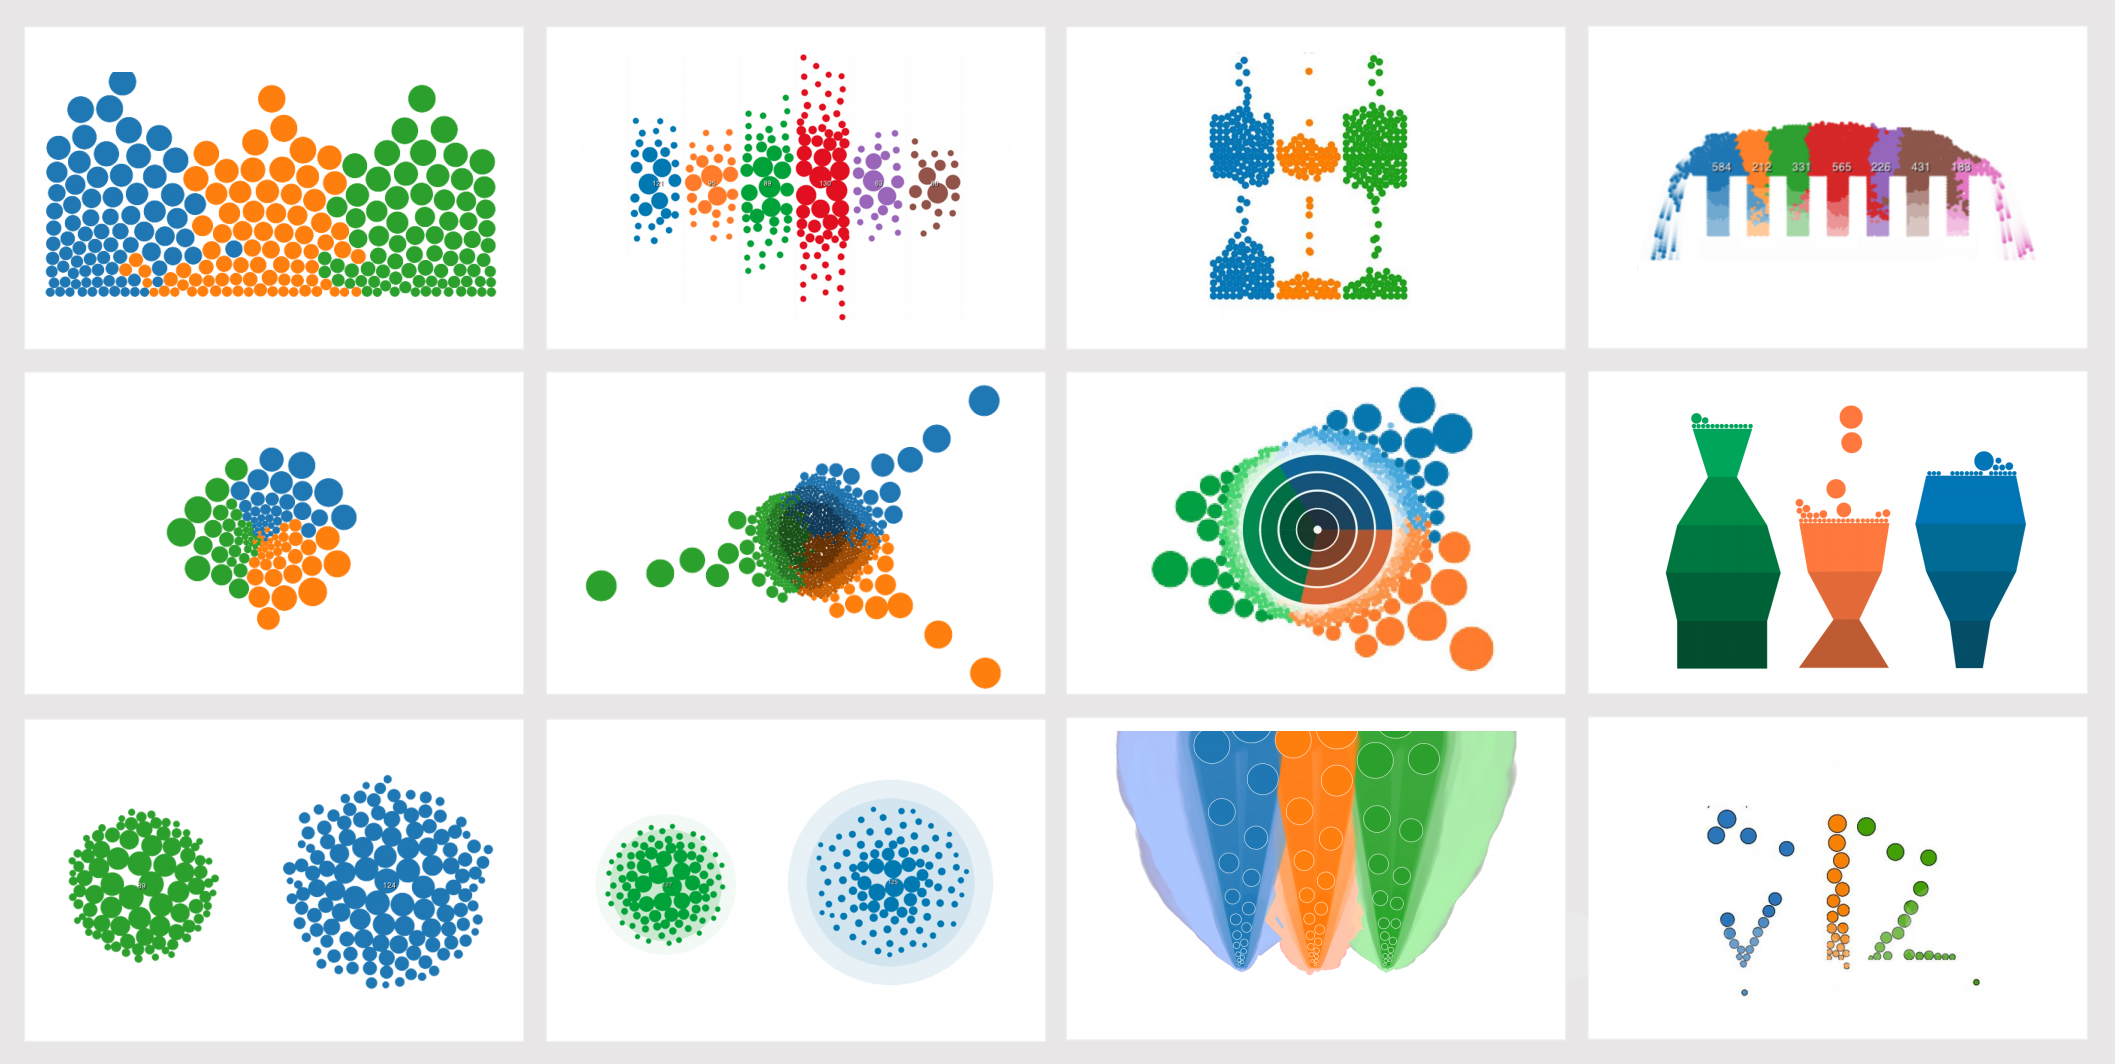
\includegraphics[height=5cm]{images/methods/related/visual-sedimentation}
\caption[
    Charts created by visual sedimentation \iacite{Huron2013}.
]{Charts created by visual sedimentation}
\label{fig:visual-sedimentation}
\end{figure}

Figure \ref{fig:visual-sedimentation} on page \pageref{fig:visual-sedimentation} shows possible charts made by visual sedimentation.

% 1, evtl. 2 with self contribution


\subsubsection{FluxFlow}
temp \iacite{Zhao2014}

\subsubsection{Gapminder}
temp

\subsubsection{Excel}
temp

\subsubsection{Tableau}
temp \iacite{Murray2013}


% WHY TASK ABSTRACTION
% Figure 3.3. Name Voyager, a vis tool originally intended for parents focused deciding on what to name their expected
% baby, ended up being used by many nonparents to analyze historical trends for their own enjoyment. Left: Names
% starting with ‘O’ had a notable dip in popularity in the middle of the century. Right: Names starting with ‘LAT’ show
% a trend of the 1970s. After [Wattenberg 05, Figures 2 and 3], using http://www.babynamewizard.com.